\documentclass[a4paper, 12pt]{report}

\usepackage[dvipsnames]{xcolor}

%%%%%%%%%%%%%%%%
% Set Variables %
%%%%%%%%%%%%%%%%

\def\useItalian{0}  % 1 = Italian, 0 = English

\def\courseName{Autonomous Networking}

\def\coursePrerequisites{Sufficient knowledge of computer networks, algorithms and probability}

\def\book{\curlyquotes{Reinforcement Learning: An Introduction}, R. S. Sutton, A. G. Barto}

\def\authorName{Simone Bianco}
\def\email{bianco.simone@outlook.it}
\def\github{https://github.com/Exyss/university-notes}
\def\linkedin{https://www.linkedin.com/in/simone-bianco}

%%%%%%%%%%%%
% Packages %
%%%%%%%%%%%%

\usepackage{../../packages/Nyx/nyx-packages}
\usepackage{../../packages/Nyx/nyx-styles}
\usepackage{../../packages/Nyx/nyx-frames}
\usepackage{../../packages/Nyx/nyx-macros}
\usepackage{../../packages/Nyx/nyx-title}
\usepackage{../../packages/Nyx/nyx-intro}

%%%%%%%%%%%%%%
% Title-page %
%%%%%%%%%%%%%%

\logo{../../packages/Nyx/logo.png}

\if\useItalian1
    \institute{\curlyquotes{\hspace{0.25mm}Sapienza} Università di Roma}
    \faculty{Ingegneria dell'Informazione,\\Informatica e Statistica}
    \department{Dipartimento di Informatica}
    \ifdefined\book
        \subtitle{Appunti integrati con il libro \book}
    \fi
    \author{\textit{Autore}\\\authorName}
\else
    \institute{\curlyquotes{\hspace{0.25mm}Sapienza} University of Rome}
    \faculty{Faculty of Information Engineering,\\Informatics and Statistics}
    \department{Department of Computer Science}
    \ifdefined\book
        \subtitle{Lecture notes integrated with the book \book}
    \fi
    \author{\textit{Author}\\\authorName}
\fi


\title{\courseName}
\date{\today}

% \supervisor{Linus \textsc{Torvalds}}
% \context{Well, I was bored\ldots}

%%%%%%%%%%%%
% Document %
%%%%%%%%%%%%

\addbibresource{./references.bib}

\begin{document}
    \maketitle

    % The following style changes are valid only inside this scope 
    {
        \hypersetup{allcolors=black}
        \fancypagestyle{plain}{%
        \fancyhead{}        % clear all header fields
        \fancyfoot{}        % clear all header fields
        \fancyfoot[C]{\thepage}
        \renewcommand{\headrulewidth}{0pt}
        \renewcommand{\footrulewidth}{0pt}}

        \romantableofcontents
    }

    \introduction

    %%%%%%%%%%%%%%%%%%%%%

    \chapter{Autonomous wireless systems}

    \section{Autonomous networks}

    With the exponential growth in the use of electronic devices, the emplyment of autonomous networks naturally increased. These type of networks revolve around four main characteristics:
    \begin{itemize}
        \item \textbf{Self-governance}: they don't require human interventions, making independent decision based on predefined rules and real-time data
        \item \textbf{Self-sufficiency}: they exist and function as an independent organism capable of managing its own resources and processes
        \item \textbf{Embedded intelligence}: they use advanced algorithms and artificial intelligence to interpret envitonmental inputs, learn from past experiences and adapt to changing conditions
        \item \textbf{Practive response}: they continuously monitor the environment, anticipate changes and react autonomously to maintain optimal performance and reliability
    \end{itemize}

    To achieve autonomous networks, \textit{wireless technologies} are preferred due to their natural independence between each other: if there is no cable connecting two devices then the two devices can freely interact with the environment.

    The main examples of such wireless technologies involve \textit{Radio Frequency Identification (RFID)} devices, \textit{sensor networks} and \textit{smart devices}.

    While designing autonomous networks, we address \textit{autonomy} mainly at the networking level (communication and routing), but also in mobility. In modern days, the best answer for such task it \textbf{reinforcement learning}, which can be summarized as all the set of techniques that can be used to determine how an intelligent agent can learn to make a good sequence of decisions. In this chapter we'll discuss the main wireless technologies that can be used in autonomous networks. In the following one, we'll discuss how reinforcement learning can be applied to such technologies in order to solve a networking problem.

    \section{Radio Frequency Identification (RFID)}

    \textbf{Radio Frequency Identification (RFID)} is a technology that uses radio frequencies in order to uniquely identify and track objects, people and animals. RFID communications are based on three components:
    \begin{itemize}
        \item \textbf{RFID tag} (or \textit{transponder}): devices that contain a chip with an embedded unique identifier (they may also be provided with some memory chips). The chip may be \textit{passive} (no battery required) or \textit{active} (battery required)
        \item \textbf{RFID reader} (or \textit{interrogator}): devices that send radio signals in order to activate RFID tags and read their informations
        \item \textbf{Managing system}: a server that handles the data received by the readers
    \end{itemize}

    Tags are typically implemented through very small chips, while readers consist of more powerful devices provided with antennas. RFID object identification has many applicaations, from inventory and logistics to domots and assisted living.

    There are two main types of RFID communication: reader-to-tags and tags-to-reader. In these communications, passive tags reflect the high-power constant signal generated by the reader, embedding their ID and info inside the reflected signal (\textbf{backscattering}), typically containing 96 bits of information (max 256 bits).

    \begin{figure}[H]
        \centering
        \includegraphics[scale=0.3]{images/backscattering.png}
        \caption{Description of RFID communication.}
    \end{figure}

    The RFID communication channel is, by definition, shared among all devices. In fact, the system is very susceptible to \textbf{collisions}: if multiple tags are reached by the signal of the same reader, they'll simultaneously reply. Collisions aren't the only issue in RFID communications. In fact, by construction of the system itself it is clear that tags outnumber readers with a large margin. This raises the problem of identification among tags with the least amount of data needed. Moreover, tags cannot ear each other since they have no \textit{carrirer sense} and no \textit{collision detection}, implying that the reader is in charge of managing the \textbf{channel access} all by itself.

    Several \textbf{Media Access Control (MAC)} protocols have been proposed to identify tags in a RFID system. Sequential MAC protocols for RFID systems aim at distinguishing tag transmissions through a specific serial number (\textbf{singulation}). There are two main types of sequential protocols: \textit{tree based protocols} and \textit{aloha based protocols}.

    \subsection{Tree based MAC protocols}

    The first tree based MAC protocol for RFID communications that we'll discuss is the \textbf{Binary Splitting  (BS)} protocol. The BS protocol recursively splits answering tags into two subgroups until it obtains single-tag groups. Tags answer to reader's queries according to the generation of a binary random number.

    Suppose that we have a set of tags to identify. Each tag has a counter initially set to zero. Each time the counter of a tag is set to 0, it will reply to the reader's query.
    \begin{enumerate}
        \item The reader sends a query. All tags whose counter is set to 0 will reply.
        \item If more than one tag replies, the reader sends a collision message. Each tag that replied before the collision generates a random bit, summing it to their own counter. Each tag that didn't reply, instead, increases its counter by 1 by default.
        \item If at most one tag replies (no collision), all tags decrement their counter by 1 (the minimum value for the counter is 0).
        \item The process is repeated from step 1 until all tags are identified
    \end{enumerate}

    Consider the following example. Suppose that we have a set $S_0$ of 8 tags to identify. Initially, the counter of each tag is set to 0, hence they all reply. After the collision, some tags will have the counter set to 0 (subgroup $S_1$), while the others will have the counter set to 1 (subgroup $S_2$).

    \begin{figure}[H]
        \centering

        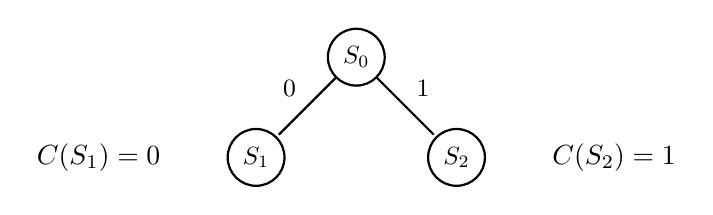
\begin{tikzpicture}[-,>=stealth,shorten >=1pt,auto,node distance=2cm, thick,main node/.style={scale=0.9,circle,draw,font=\sffamily\normalsize}]

            \node[main node] (0) []{$S_0$};
            \node[main node] (1) [below left of = 0]{$S_1$};
            \node[main node] (2) [below right of = 0]{$S_2$};
            \node[] (c1) [left of = 1]{$C(S_1) = 0$};
            \node[] (c2) [right of = 2]{$C(S_2) = 1$};

            \path[every node/.style={font=\sffamily\small}]
                (0) edge [swap] node{$0$} (1)
                (0) edge node{$1$} (2)
                ;
        \end{tikzpicture}
    \end{figure}
    
    On the second iteration, tags in group $S_1$ will reply the next reader's query, forming another split into two sets $S_3$ (counter set to 0) and $S_4$ (counter set to 1), while the counter of the tags in the set $S_2$ gets set to 2. 

    \begin{figure}[H]
        \centering

        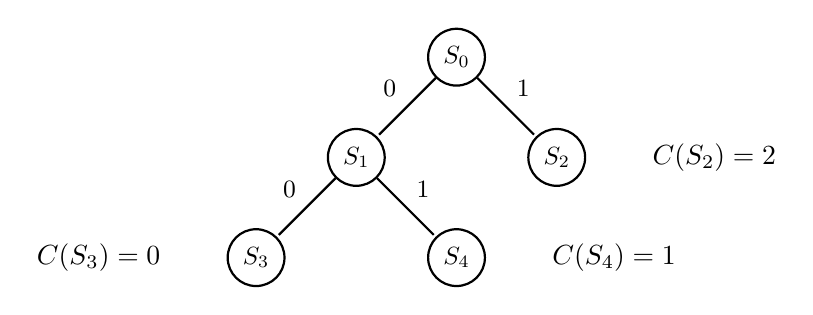
\begin{tikzpicture}[-,>=stealth,shorten >=1pt,auto,node distance=2cm, thick,main node/.style={scale=0.9,circle,draw,font=\sffamily\normalsize}]

            \node[main node] (0) []{$S_0$};
            \node[main node] (1) [below left of = 0]{$S_1$};
            \node[main node] (2) [below right of = 0]{$S_2$};
            \node[main node] (3) [below left of = 1]{$S_3$};
            \node[main node] (4) [below right of = 1]{$S_4$};
            \node[] (c3) [left of = 3]{$C(S_3) = 0$};
            \node[] (c2) [right of = 4]{$C(S_4) = 1$};
            \node[] (c2) [right of = 2]{$C(S_2) = 2$};

            \path[every node/.style={font=\sffamily\small}]
                (0) edge [swap] node{$0$} (1)
                (0) edge node{$1$} (2)
                (1) edge [swap] node{$0$} (3)
                (1) edge node{$1$} (4)
                ;
        \end{tikzpicture}
    \end{figure}

    Suppose now that in the third iteration $S_3$ contains only one tag. Since the will be no collision, this unique tag will be correctly identified by the reader. Then, the counters of $S_4$ and $S_2$ get decreased by 1 since a tag has been identified.

    \begin{figure}[H]
        \centering

        \begin{tikzpicture}[-,>=stealth,shorten >=1pt,auto,node distance=2cm, thick,main node/.style={scale=0.9,circle,draw,font=\sffamily\normalsize}]

            \node[main node] (0) []{$S_0$};
            \node[main node] (1) [below left of = 0]{$S_1$};
            \node[main node] (2) [below right of = 0]{$S_2$};
            \node[main node, accepting] (3) [below left of = 1]{$S_3$};
            \node[main node] (4) [below right of = 1]{$S_4$};
            \node[] (c2) [right of = 4]{$C(S_4) = 0$};
            \node[] (c2) [right of = 2]{$C(S_2) = 1$};

            \path[every node/.style={font=\sffamily\small}]
                (0) edge [swap] node{$0$} (1)
                (0) edge node{$1$} (2)
                (1) edge [swap] node{$0$} (3)
                (1) edge node{$1$} (4)
                ;
        \end{tikzpicture}
    \end{figure}
    
    The fourth iteration then proceeds on $S_4$ and will eventually proceed also on $S_2$. In general, the binary splitting protocol can be viewed as a depth-first search that prioritizes tags whose counter is currently set to 0. Binary splitting works good on average. However, the use of random counter increments may yield cases with a non optimal split (i.e. most of the tags may fall in the same set), requiring multiple splits.

    A more simple protocol based on this idea is the \textbf{Query Tree (QT)} protocol. Here, tags are queried according the the binary structure of their IDs (recall that each tag typically has an ID of 96 bits):
    \begin{enumerate}
        \item The reader queries all tags by sending a binary string. Only the tags whose ID have a prefix matching the string answer the query
        \item The string is initially set to the empty string $\varepsilon$.
        \item If more than one tag replies (collision), the reader recursively makes two queries. The first query extends the string with a 0, while the second extends the string with a 1.
        \item If at most one tag replies (no collision), the corresponding branch of the protocol gets killed.
    \end{enumerate}

    \begin{figure}[H]
        \centering

        \begin{tikzpicture}[-,>=stealth,shorten >=1pt,auto,node distance=2cm, thick,main node/.style={scale=0.9,circle,draw,font=\sffamily\normalsize}]

            \node[main node] (0) []{$\varepsilon$};
            \node[main node] (1) [below left of = 0]{$0$};
            \node[main node, accepting] (2) [below right of = 0]{$1$};
            \node[main node] (3) [below left of = 1]{$00$};
            \node[main node] (4) [below right of = 1]{$01$};
            \node[main node, accepting] (5) [below left of = 4]{$010$};
            \node[main node, accepting] (6) [below right of = 4]{$011$};

            \path[every node/.style={font=\sffamily\small}]
                (0) edge [swap] node{$0$} (1)
                (0) edge node{$1$} (2)
                (1) edge [swap] node{$0$} (3)
                (1) edge node{$1$} (4)
                (4) edge [swap] node{$0$} (5)
                (4) edge node{$1$} (6)
                ;
        \end{tikzpicture}

        \caption{Tree generated by the QT protocol for the IDs $0100, 0111$ and $1010$}
    \end{figure}
    
    In case of uniform distribution, the tree induced by BT and QT are almost the same due to each split having the same expected size. To measure performance of RFID protocols, we want to determine how fast a protocol is to collect all tags ID. If we have $n$ tags, the protocoll will end when all $n$ tags have responded singularly. The \textbf{system's efficiency} is measured as the ratio between the number of tags $n$ and the number of queries $q$.
    \[\mathrm{SE} = \frac{n}{q}\]

    When $n = q$, the protocol is clearly optimal. However, in practice the SE value is far below 1. For instance, consider the BS protocol. To evaluate $\mathrm{SE}_{\mathrm{BS}}$, we need to estimate the total number of queries for $n$ tags, denoted with $\mathrm{BS}_{\mathrm{tot}}(n)$. We observe that on each query the tag set is split into two sets, one with $k$ elements and one with $n-k$ elements, giving the following recursive equation.
    \[\mathrm{BS}_{\mathrm{tot}}(n) = \soe{ll}{
        1 + \sum_{k = 0}^n \binom{n}{k} \rbk{\frac{1}{2}}^k \rbk{1-\frac{1}{2}}^{n-k}(\mathrm{BS}_{\mathrm{tot}}(k) + \mathrm{BS}_{\mathrm{tot}}(n-k)) & \text{if } n > 1 \\
        1 & \text{otherwise}
    }\]

    For large values of $n$ we get that:
    \[\lim_{n \to +\infty} \mathrm{SE}_{\mathrm{BS}} = \lim_{n \to +\infty} \frac{n}{\mathrm{BS}_{\mathrm{tot}}(n)} \approx 0.38\]

    \subsection{Aloha based MAC protocols}

    In Aloha based protocols, time is \textit{slotted}. On each slot, at most one tag can communicate (slot duration is equal to the tag's ID transmission time). Slots are grouped into frames, where each tag randomly picks a slot.

    In \textbf{Framed Slotted Aloha (FSA)}, when the reader issues a start of a frame, it includes the number of $N$ slots in such frame. The $n$ tags randomly pick a slot of the frame. If a collision occurs, i.e. two tags try to communicate in the same slot, the process repeats is reapplied on all the tags that have collided, until all tags are identified.

    \begin{figure}[H]
        \centering
        \includegraphics[scale=0.5]{images/fsa.png}
        \caption{The FSA protocol in action (6 total slots with 3 collisions and 3 identifications).}
    \end{figure}

    In general, the FSA protocol reaches the best performance when the number of slots in a frame is equal to the number of tags to be identified, i.e. when $N = n$, achieving a 37\% of identification slots and 63\% of collision slots. 

    In particular, the probability that $r$ out of $n$ tags answer in the same slot among $N$ slots is given by the binomial distribution:
    \[\Pr[\text{$r$ tags in same slot}] = \binom{n}{r} \rbk{\frac{1}{N}}^r \rbk{1-\frac{1}{N}}^{n-r}\]
    implying that the number $s(r)$ of slots with exactly $r$ tags is expected to be:
    \[s(r)= N \binom{n}{r} \rbk{\frac{1}{N}}^r \rbk{1-\frac{1}{N}}^{n-r}\]

    Let $R_{\mathrm{idle}}, R_{\mathrm{id}}, R_\mathrm{col}$ be the number of identification, collision and idle rounds during the tag identification process. It's easy to see that:
    \[R_{\mathrm{idle}} = N \rbk{1-\frac{1}{N}}^n \quad R_{\mathrm{id}} = n \rbk{1-\frac{1}{N}}^{n-1} \quad R_{\mathrm{col}} = N - R_{\mathrm{idle}} - R_{\mathrm{id}}\]

    The system's efficiency in this case is given by:
    \[\mathrm{SE}_{\mathrm{FSA}} = \frac{R_{\mathrm{id}}}{R_{\mathrm{idle}} +  R_{\mathrm{id}} + R_\mathrm{col}}\]

    In case of rounds of the same exact duration, this value tends to 37\%.

    The \textbf{Electronic Product Code Generation 2 (EPC Gen 2)} standard is a protocol based on FSA. EPC adapts frame length according to the number of collision and empty slots. In particular, EPC Gen 2 specifies the \textbf{transmission time model}, which allows us to estimate a temporal evaluation of the protocol's performance.

    The key aspect behind this model stands in observing that \textit{idle responses}, i.e. slots where no tag answers, can last less than identification or colliding responses because the tags don't have to reply to the reader.

    \begin{figure}[H]
        \centering
        \includegraphics[scale=0.75]{images/trans_time_model_1.png}

        \includegraphics[scale=0.75]{images/trans_time_model_2.png}

        \caption{The two types of slots used by the EPC Gen 2 standard.}
    \end{figure}

    Hence, if idle rounds last a $\beta$ faction of the identification and collision rounds, we get that:
    \[\mathrm{TimeSE}_{\mathrm{FSA}} = \beta \frac{R_{\mathrm{id}}}{R_{\mathrm{idle}} +  R_{\mathrm{id}} + R_\mathrm{col}} = \frac{n \rbk{1-\frac{1}{N}}^{n-1}}{(\beta-1) N \rbk{1-\frac{1}{N}}^n + N}\]

    \begin{figure}[H]
        \centering
        \includegraphics[scale=0.5]{images/trans_time_model_3.png}

        \caption{Performance comparison with and without the transmission time model.}
    \end{figure}

    From the above graph, we observe that the best performance is reached with the transmission time model. In particular, we observe that when the number of tags is known, the amount of collisions can be drastically reduced (initially) by setting $N = n$. On average, this new version of FSA wastes 40\% of the time slots in idle and collision slots.

    This number can be further improved through a mode complex protocol, that being the \textbf{Tree Slotted Aloha (TSA)} protocol. In this variant, slots are executed following a tree: a new \textit{child frame} is issued for each collision slot, where only the tags in the same slot participate in the new child frame.

    \begin{figure}[H]
        \centering
        \includegraphics[scale=0.5]{images/treeslot_aloha.pdf}

        \caption{The TSA protocol in action. Green squares represent identifications, red squares represent collisions and white squares represent idle rounds.}
    \end{figure}

    To estimate the performance of the TSA protocol, we count the number of nodes in a fashion similar to the BS protocol:

    \[\mathrm{TSA}_{\mathrm{tot}}(n) = \soe{ll}{
        1 + \sum_{k = 0}^n \binom{n}{k} \rbk{\frac{1}{2}}^k \rbk{1-\frac{1}{2}}^{n-k}\mathrm{TSA}_{\mathrm{tot}}(k) & \text{if } n > 1 \\
        1 & \text{otherwise}
    }\]

    
    For large values of $n$ we get that:
    \[\lim_{n \to +\infty} \mathrm{SE}_{\mathrm{TSA}} = \lim_{n \to +\infty} \frac{n}{\mathrm{TSA}_{\mathrm{tot}}(n)} \approx 0.42\]

    \subsection{Estimating tag population}

    In order for a RFID communication protocol to be effective, it must work with a potentially infinite number of tags. This makes the initial number of tags unknown to the RFID reader. Initial frame size is usually set to a predefined value (typically 128 slots), while the size of the subsequent frames is computed through the output of the following formula:
    \[\text{tags per collision slot} = \frac{\text{estimated tot. num. of tags } - \text{ identified tags}}{\textit{collision slots}}\]

    The number of identified tags and number of collision slots is known, but we dont know the total number of tags. This last value is estimated according to the outcome of the previous frame using Chebyshev's inequality. Let:
    \begin{itemize}
        \item $N$ be the size of the previous frame
        \item $(c_0, c_1, c_k)$ be a triple of observed values
        \item $(a_0, a_1, a_k)$ be a triple of estimated values
    \end{itemize}

    The \textbf{estimator function} $\varepsilon$ is defined as:
    \[\varepsilon(N,c_0,c_1,c_k) = \min_{n \in [c_1+2c_k, 2(c_1+2c_k)]} \abs{\smat{a_0^{N,n} \\ a_1^{N,n}} \\ a_k^{N,n} - \smat{c_0 \\ c_1} \\ c_k} \]

    where $a_r^{N,n}$ is the expected number of slots with $r$ tags:
    \[a_{r}^{N,n} = N \binom{n}{r} \rbk{\frac{1}{N}}^r \rbk{1-\frac{1}{N}}^{n-r}\]

    We observe that the estimator function doesn't capture the possibility of high variance in the number of tags. We also observe that the upper bound $2(c_1+2c_k)$ is not adequate for networks composed of thousands of nodes. For instance, if we have 5000 tags with $N = 128$, it is highly likely that for $c_1 = 0$ the upper bound is estimated as $2(c_1+2c_k) = 512$, which is definitely to small. However, an \textit{unbounded estimator} can still be not accurate.
    
    The key observation here lies in the fact that starting with a proper frame size leads to better estimations for intermediate frames (improved convergence). Hence, the problem can be compressed into estimating the initial tag population to properly set the size of the first frame. The two common solutions for this task are the \textit{Dy\_TSA protocol} and the \textbf{Binary Splitting Tree Slotted Aloha (BSTSA)}. The latter protocol uses BS to randomly split tags into groups whose size can be easily estimated and then use TSA in these groups.

    \begin{figure}[H]
        \centering
        \includegraphics[scale=0.4]{images/bstsa.png}

        \includegraphics[scale=0.4]{images/bstsa_2.png}
        \caption{The BSTSA protocol in action and its performance compared to other protocols.}
    \end{figure}

    \newpage

    \section{Wireless Sensor Networks (WSN)}

    In wireless networks, sensors are devices provided with battery that continuously sense the environment, listening on the channel (\textit{carrier sense}) and spontaneously transmitting information (\textit{no backscattering}) when something is sensed. The device receiving the information of multiple sensors is often referred to as \textit{sink}. In particular, we observe that, very differently from RFID tags, sensors can achieve complex computations. Moreover, multi-hop communication is also possible: sensors can exchange information either through the sink or by communicating directly with each other.
    
    Formally, a \textbf{Wireless Sensor Network (WSN)} is a sensor networks composed of distributed devices that monitor and record environmental conditions, sending the discovered data to a central node for processing and analysis. The central node may then send a signal to a control device that takes action regarding the gathered information.
    
    \begin{figure}[H]
        \centering
        \includegraphics[scale=0.5]{images/wsn.png}
        \caption{Example of a WSN with sensors that measure humidity in order to detect weather changes.}
    \end{figure}
    
    Sensor networks have multiple benefits compared to other architectures:
    \begin{itemize}
        \item \textbf{Large-scale coverage}: they can collect data across vast geographic areas, even in remote or inaccessible locations.
        \item \textbf{Autonomous operation}: each sensor is independent from the others, minimizing the need of human intervention
        \item \textbf{Real-time data}: their simplicity allows immediate access to critical data, enabling rapid response to environmental changes
    \end{itemize}

    For these reasons, WSNs are emplyed \underline{everywhere} there is a need for monitoring a physical space or using sensors for controlling a procedure (e.g. industrial control, marine monitoring, health care, smart homes, structural health, \dots).
    
    We categorize devices taking part in a WSN in three main types: \textbf{sources} of data (\textit{sensors}), \textbf{sinks} of data (\textit{central nodes}) and \textbf{actors} (\textit{control devices}). To deploy sensors, there are three main methods:
    \begin{itemize}
        \item \textbf{Random deployment}: sensors are dropped from aircraft using an uniform at random distribution over the area
        \item \textbf{Regular deployment}: sensors are disposed in a well planned schema, not necessarily resembling a geometric structure (often assumed to be for cost efficiency, even when false).
        \item \textbf{Mobile sensors}: sensors can autonomously move according to a distributed algorithm, compensating uncovered areas. They can be passively moved around by some external force (wind, water, \dots) or actively seek our areas of interest
    \end{itemize}

    In particular, mobile sensors deployment rose in recent years due to the introduction of network paradigms based on continuously changing and adapting topologies, instead of fixed ones. However, all types of WSNs come with some issues that must be mitigated:
    \begin{itemize}
        \item \textbf{Information content}: data must be processed in-network and it must provide answers to queries or events triggered by sensors. This implies that there is an asymmetric flow of information inside the network (sensors to sink).
        \item \textbf{Quality of service}: traditional network QoS metrics do not apply in sensor networks.
        \item \textbf{Fault tolerance}: the network must be robust against node failure, which may happen more commonly due to sensors being fragile.
        \item \textbf{Energy consumption}: sensors networks must achieve their task for as long as possible, making energy one of the main issues due to the low resources available and the necessity for continuous data gathering. This is the main critical issue in WSNs.
    \end{itemize} 

    Sensor nodes are composed of few components: a CPU, a memory unit, a power source (usually a battery), an antenna, a radio frequency transceiver and a sensor unit. Alls these components are managed through a standard operating system called TinyOS, initially developed by the University of California. Sensor units capture a signal corresponding to a physical phenonmenon, which then gets prepared for further use through \textit{signal conditioning} (e.g. amplification, attenuation, filtering, \dots) and converted from analog to digital.
    
    To mitigate energy consumption, sensors are constructed in an energy efficiency principle: sensor networks are typically deployed in an ad hoc fashion, with individual nodes remaining largely inactive for long periods of time, but then becoming suddenly active when something is detected (\textbf{trigger}). Nonetheless, some energy is wasted by nature of the sensors themselves:
    \begin{itemize}
        \item Collisions may force the sensors to retrasmit information
        \item A node may receive packets that are meant for other nodes (\textbf{overhearing})
        \item A minimal number of control packets must be used for data transmissions
        \item Nodes must be constantly listening to an idle channel in order to get triggered
        \item A node may transmit packets to a node that is currently busy (\textbf{overemitting})
    \end{itemize} 

    Along with energy consumption, WSNs share the same wireless communication criticall issues as any other wireless network:
    \begin{itemize}
        \item \textbf{Attenuation}: the electromagnetic signals decreases rapidly as the distance from the transmitter increases (the signal is dispersed in all directions).
        \item \textbf{Multi-path propagation}: when a radio-wave hits an obstacle, part of the wave is reflected with a loss of power. This implies that a source signal may arrive at the same destination multiple times through multiple reflections.
        \item \textbf{Interference}: a recipient can receive multiple signals from the desired sender due to multi-path propagation or from multiple trasmitters that are using the same frequency to communicate with other recipients (e.g. Wi-Fi, Bluetooth and Microwaves all share the same frequency range).
    \end{itemize} 

    These issues are measured through \textbf{Signal-to-Noise Ratio (SNR)}, the ratio between good (signal) and bad (noise) signals received by a device. When the SNR is high, the signal is stronger than the noise. When low, the amount of noise is greater. 

    Furthermore, there are some inheritent issue that arise in wireless communication due to its very own nature such as the \textbf{Hidden Terminal Problem (HTP)}: two nodes $A$ and $B$ may be communicating with the same device $B$ without knowing the existence of each other, forming collisions in the network.

    From the above discussion, it should be clear that the key to mitigating both energy consumption and wireless issues lies in the MAC protocols used by the sensors. In particular, WSN MAC protocols must control \textit{when} a packete must be sent and \textit{when} a packet must be listened. All protocols for sensor networks are based on two communication patters that alternate between each other:
    \begin{itemize}
        \item \textbf{Broadcast} (or \textit{Interest Dissemination}): the sink transmits information to all sensors in the network (One-to-All), typically used to send queries, update sensors and control packets
        \item \textbf{Convergecast} (or \textit{Data Gathering}): a subset of sensors nodes send data to the sink (Many-to-One), typically used for collecting sensed data
    \end{itemize}

    WSN MAC protocols are based on one of two techniques: \textbf{contention} and \textbf{scheduling}. In the former, on-demand allocation is used for nodes that have information to transmit, managing collisions when they occur. In the latter, the sink specifies when and for how long each node may transmit over the shared channel. Contention based protocols are more scalable but less energy efficient, while scheduling based ones are more energy efficient but require a synchronization and a central authority in the network.

    \section{Contention-based MAC protocols for WSN}

    \subsection{CSMA/CA protocol}

    The first type of contention based MAC protocols that we'll discuss is the \textbf{CSMA/CA} protocol, defined by the IEEE 802.11 standard. Here, CSMA/CA stands for \textbf{Carrier Sense Multiple Access with Collision Avoidance}, implying that the protocol \underline{cannot detect} collision, but it can only try to avoid them as much as possible (a more advanced protocol, the CSMA/CD, is capable of doing so). 

    When a node wants to transmit a frame, it first \textit{senses} the channel for a small time slot called \textbf{interframe space (IFS)}. If the channel is \textit{idle}, i.e. no device transmits during the sensing period, the device immediately trasmits when the IFS ends.
    
    Otherwise, if the channel is busy, the station continues to monitor the channel until the transmission ends. Once the transmission is over, the station delays another IFS. Then, the node enters a \textit{contention window} with the other nodes, where each of them waits for a randomly chosen amount of time (\textbf{back-off phase}).
    
    The \curlyquotes{luckiest} node whose wait time expires first will be the first one to return to the sensing phase, making it the first one to trasmit. The back-off clock of each node is randomly chosen from the range $[0, \mathrm{CW}-1]$. In the \textit{binary exponential back-off}, the value of $\mathrm{CW}$ is doubled each time the node enters the back-off phase, getting reset to the initial value when the node successfully transmits.

    \begin{figure}[H]
        \centering
        \includegraphics[scale=0.5]{images/csma_ca.png}
        \caption{The CSMA/CA protocol in action.}
    \end{figure}

    Advanced versions of CSMA/CA use different type IFS in order to dictate priorities among nodes. In particular, \textbf{Short IFS (SIFS)} are used for packets of the highest priorities while \textbf{Distributed coordination function IFS (DIFS)} are are used for packets of the lowerst priorities and asynchronous data services. DIFS are usually as long as a SIFS plus two time slots.
    
    In \textit{Distributed coordination function CSMA/CA with Acknowledgement} (DFS CSMA/CA ACK), each station has to wait a DIFS before sending data (instead of a generic IFS). When the destination receives the data, it waits for a SIFS and then immediately sends an ACK message (without sensing the channel) if the packet was correctly received. If the ACK is lost, the trasmission is repeated. Otherwise, the sending node waits a DIFS and then enters the contention window.

    The CSMA/CA protocol suffers from not only the Hidden Terminal Problem, but also from the \textit{Exposed Terminal Problem}, a similar problem that forms when a terminal's communication is postponed by the carrier sense even though no collision would happen.

    \begin{figure}[H]
        \centering
        \includegraphics[scale=0.5]{images/htp_2.png}
        \caption{Since the nodes $A$ and $C$ cannot hear each other, when $A$ transmits to $B$, $C$ cannot sense the transmission. Hence, $C$ may transmits to $D$ during this time slot, forming a collision for $B$.}
    \end{figure}

    \begin{figure}[H]
        \centering
        \includegraphics[scale=0.5]{images/etp.png}
        \caption{Since $B$ and $D$ cannot hear each other, $B$ may transmit to $A$ while $C$ may transmit to $D$ without creating a collision. However, when $B$ tries to transmit to $A$, it may detect the channel as occupied by $C$, postponing the transmission.}
    \end{figure}

    To solve these two issues, DCF CSMA/CA can be further extended with two new control packets. After waiting the DIFS, the transmitting node first sends a \textbf{Request-To-Send (RTS)} packet. After receiving the RTS message, the receiving node waits a SIFS and then sends a \textbf{Clear-To-Send (CTS)} packet if it didn't sense anything on the channel. Once the CTS message is received, the two devices proceed with the transmission as previously defined.

    \begin{figure}[H]
        \centering
        \includegraphics[scale=0.5]{images/csma_ca_rts_cts.png}
        \caption{The DCF CSMA/CA with ACK and RTS/CTS in action.}
    \end{figure}

    The RTS/CTS packets are used to reserve the channel for data transmission, solving both the HTP and the ETP (when a node receives a CTS without sending a RTS, it ignores the CTS message). Moreover, this procedure also makes it impossible for collision to happen during transmission since only two devices can communicate in the same time slot. However, collision \textit{is} still possible: the RTS packets sent by multiple devices may collide. However, these collisions are not as bad as data collisions since RTS packets are much smaller.
    
    The DCF CSMA/CA with ACK and RTS/CTS defined in the IEEE 802.11 standard empyes both a \textit{physical} carrier sense and a \textit{virtual} carrier sense. The latter is provided by the \textbf{Network Allocation Vector (NAV)}. When the correct destination receives a RTS message, it embeds a NAV value in the CTS message sent as an answer. This NAV value defines the amount of time for which the receiver expects the communication to last.
    
    During the transmission, nodes that aren't involved start counting down from NAV to 0. As long as the NAV $> 0$, the channel is considered busy. Each time the channel is virtually available, the MAC protocol checks if it is also physically available. This process highly reduces the amount of time each device spends physically sensing the channel. 

    \subsection{S-MAC protocol}

    The second type of contention based MAC protocols that we'll discuss is the \textbf{S-MAC} protocol. Here, S-MAC stands for \textbf{Sleep MAC}. This protocol tries to reduce energy waste in echange for some performance reduction due to latency. Since \textit{idle listening} is the principal source of energy waste, S-MAC tries to mitigate this problem by alternating sensing phases with \textbf{sleep phases}, where the radio component of the device is turned off.

    Since sensor devices have to be constantly active, the employment of even a small amount of sleep phases is good enough to highly reduce energy waste. For instance, listening for 200ms and then sleeping for 2s reduces the \textbf{duty cycle} by 10\%. The duty cycle is formally defined as the ratio beween the listening interval and the frame duration (listening + sleeping). 
    
    Each node is free to choose their own listen/sleep schedules. But what if a node wants to communicate with another node that is currectly sleeping? To fix this issue, \textbf{periodic synchronization} is used among nodes: neighboring nodes are synchronized together, meaning that they use the same listen/sleep schedules. If two nodes are neighbors are part of two different virtual clusters, a common sleep schedule may be also used.

    \begin{figure}[H]
        \centering
        \includegraphics[scale=0.6]{images/smac.png}
        \caption{S-MAC schedule tables among the networks.}
    \end{figure}

    Every node of the network maintains a table containing its neighbors' schedules. Each entry is filled (or updated) when the node receives a \textbf{SYNC packet}, which contains the sender nodes's ID and the next interval in which he's going to sleep. If no interval is specified in the received message, the destination will fill the entry with a random interval.

    A more careful approach has to be used for the initial schedule of each node, due to each table being empty:
    \begin{enumerate}
        \item A node first listens for a certain amount of time (at least the synchronization period)
        \item If no schedule is received during this phase, the node randomly chooses a schedule and immediately broadcasts its schedule with a SYNC packet. This node is referred to as the \textbf{synchronizer}.
        \item Otherwise, the node follows the received schedule and waits a random delay before broadcasting its schedule. This node is referred to as the \textbf{follower}.
    \end{enumerate}

    Clearly, this protocol cannot guarantee that in a large network all nodes will follow the same schedule. For instance, a middle node may receive a schedule from two neighbors that are following two different schedules, making it follow both of them at the same time. This also implies that whenever this middle node has to broadcast a SYNC packet, it needs to send it twice, one for each group.

    Since S-MAC is also based on contention, it suffers from collisio just as the CSMA/CA protocol. This problem is mitigated using \textbf{collision avoidance} in fashion similar to the CSMA/CA with ACK, RTS/CTS and NAV. Before transmitting, the node performs a virtual sensing phase using NAV (followed by physical sensing). If the channel is busy, the node goes to sleep and wakes up when the reicever is free (according to its schedule table). The process is then repeated from the first step. Otherwise, the node starts the transmission.

    In particular, broadcast packets (SYNC) are sent without using the RTS/CTS mechanism, while unicast packets (data) use the full RTS/CTS/ACK chain. The \textit{duration field} in each transmitted packet indicates how long the remaining transmission will be. This implies that if a node receives a packet destined to another node, it will know for how long it has to keep silent,preventing overhearing.

    \begin{figure}[H]
        \centering
        \includegraphics[scale=0.6]{images/smac_2.png}
        \caption{The S-MAC protocol in action.}
    \end{figure}

    S-MAC has proven to highly reduce the energy consumption through sleeping. However, this doesn't always imply that energy waste is reduced:
    \begin{itemize}
        \item \textbf{Light traffic load}: when few messages are sent, nodes spend most of their time listening, meaning that sleep is a key part in saving energy. 
        \item \textbf{High traffic load}: when tons of messages are sent, the time spent listening by each node is close to zero, meaning that sleep is actually a problem for the network (high latency and close to zero savings)
    \end{itemize}

    \section{Routing for WSN}

    As any network, WSNs require the use of network protocols in order to share informations. Due to the inheritent problems of WSNs, standard routing techniques must be adapted in order to minimize energy consumption and maximize the lifetime of the network. Ad hoc WSN routing protocols are required for the two main topologies of WSN network, i.e. \textit{flat} and \textit{hierarchical}. For our purposes, we'll focus on flat networks.

    \textbf{Flat networks} routing protocols can be classified, according to the \textit{routing strategy}, into three main different categories depending on \underline{when} the routing protocol operates:
    \begin{itemize}
        \item \textbf{Proactive protocols} (or  \textit{table-driven protocols} ): the protocol always tries to keep its routing data up-to-date, meaning that the protocol is active before tables are actually needed.
        \item \textbf{Reactive protocols} (or \textit{on demand protocol}): the route is determine only when actually needed 
        \item \textbf{Hybrid protocols}: a combination of proactive and reactive strategies 
    \end{itemize}

    \subsection{Proactive routing}

    Proactive protocols work in a way similar to wired networks. Each node \textbf{maintains routes} to all reachable destinations at all times, whether or not there is currently any need to delived packets to those destinations.
    Hence, any time a path to some destination is needed the corresponding route is \textbf{already known}, requiring no additional time. Their proactive nature also allows them to quickly respond to any changes in network topology. However, keeping the information up-to-date may require a lot of bandwidth and extra battery power. Moreover, sometimes the information may still be out-of-date.

    The most common example of proactive routing WSN protocol is the \textbf{Destination Sequence Distance Vector (DSDV)}, an adaptation of the Distance Vector (DV) protocol typically used in wired networks. The protocol is based on a distributed computation of the Bellman-Ford routing procedure. Route updates are periodically sent or event-driven, with an additional \textit{aging} information that helps to recognize old routes, avoiding loops. Each time the topology changes, an incremental number of route updates is sent.

    Consider the following network with its initial tables. 

    \begin{figure}[H]
        \centering
        \includegraphics[scale=0.55]{images/dsdv.png}
        \caption{An example network using DSDV.}
    \end{figure}

    Suppose that node $A$ triggers a routing update, sending its table to its neighbors. Upon receiving the table, nodes $B$ and $C$ update their tables with the new information given by $A$ (e.g. $B$ now knows that it can reach $C$ through $A$ with 2 hops, one from $B$ to $A$ and one from $A$ to $C$).
    
    \begin{figure}[H]
        \centering
        \includegraphics[scale=0.55]{images/dsdv_2.png}
        \caption{The routing update triggered by $A$.}
    \end{figure}

    After updating their tables, $B$ and $C$ will also send their new tables to their neighbors. In particular, $A$ will then discover that it can reach $D$ through $C$. After another update instance, $B$ will discover than it can reach $D$ through $A$. If the topology remains unchanged, the network will eventually \textbf{converge} to fixed routing tables.

    It's easy to see that, due to its simplicity, the routing updates may form loops. Under certain conditions, these loops may force the tables to progressively increment the distance between the nodes. To avoid loops altogether, \textbf{sequence numbers} are added to each routing table entry in order to ensure that the information is fresh. Routes with higher sequence numbers are preferred as they represent more recent information.

    \subsection{Reactive routing}

    Rective protocols are source-initiated, meaning that they start a route discovery procedure only when a node requires it. This procedure is based on some form of \textit{global search} procedure. Clearly, this idea doesn't require constant updates to be sent through the network, but it also clearly causes delays due to route discovery. This discovery phase terminates when a valid route is found or when all possible routes have been examinated and declared as unavailable (due to some middle node being busy or malfunctioning).  
    
    In some cases, the desired route is kept in a route cache maintained by the sensor nodes. When this is the case, there is no additional delay. This makes reactive protocols very effective for topologies that don't change often.

    \textbf{Flooding} is an old and very simple technique also used in wired networks: copies of incoming packets are sent to every neighbor except the one who sent the packet.

    \begin{figure}[H]
        \centering

        \begin{tabular}{ccc}
            \includegraphics[scale=0.35]{images/un_broad_1.png}
            &\qquad\qquad&
            \includegraphics[scale=0.35]{images/un_broad_2.png}
        \end{tabular}

        \caption{The flooding protocol in action.}
    \end{figure}

    As long as there is a route from source to destination, the delivery of the packet is guaranteed. In particular, one copy of the packet will arrive through the quickest possible route (BFS behaviour). Due to its simplicity, flooding has many drawbacks:
    \begin{itemize}
        \item This procedure generates an enormous amount of superfluos traffic
        \item \textit{Implosion}: duplicated messages may be broadcasted to the same node
        \begin{figure}[H]
            \centering
            \includegraphics[scale=0.75]{images/implosion.png}
            \caption{Example of flooding implosion.}
        \end{figure}
        \item \textit{Data overlap}: if the observation regions of two nodes overlap, they may detect the same request simultaneously. As a result, common neighbors may receive two packets with similar information.
        \begin{figure}[H]
            \centering
            \includegraphics[scale=0.65]{images/overlap.png}
            \caption{Example of flooding data overlap.}
        \end{figure}
        \item \textit{Resource blindness}: the procedure does not take into consideration all the available energy resources. An energy resource-aware protocol must take into account the amount of energy that is available all the time.
        \item \textit{Energy consumption}: each data packet requires high energy to be broadcasted.
    \end{itemize}

    \textbf{Gossiping} is a more refined version of flooding, where the nodes send the incoming packets only to a randomly selected neighbor. Although this approach avoids the implosion problem, it takes longer to propagate the message to all sensor nodes in the network and it does not reduce the amount of consumed energy.

    Flooding and Gossiping don't use real routing algorithms since they are purely based on broadcast. A more standard routing approach is used in \textbf{Dynamic Source Routing (DSR)}, where each data packet carries in its header the complete cordered liste of nodes through which the packet will pass. The sender can select and control the routes used for its own packets, supporting the use of multiple routes to any destination. Moreover, other nodes that are forwarding or overhearing the packets can copy the header information in their cache for future use.
    
    The DSR protocol is composed of two main mechanisms that work together on demand to allow the discovery and maintainance of source routes:
    \begin{itemize}
        \item \textit{Route discovery} is the mechanism through which any node  $S$ wishing to send a packet to a destination node $D$ obtains a source route. It is used when no route from $S$ to $D$ is known.
        \item \textit{Route maintainance} is the mechanism through which any node $S$ is able to detect, while using a source route to $D$, if the network topology has changed in a way that disables the already known route. When route maintainance is triggered, $S$ can either attempt to use any of the known routes with $D$ as a destination node or invoke route discovery.
    \end{itemize}

    When route discovery is triggered, the initial node sends a \textbf{Route Request} packet, containing a unique request ID and a list of addresses, which is initialized as empty. When a node receives a request packet, it appends its own address to the list. If the intermediate node matches with the destination, it returns a \textbf{Route Reply} packet to the initial node, containing a copy of the accumulated list. Otherwise, the intermediate node then propagates the packet through a local broadcast.

    \begin{figure}[H]
        \centering
        \includegraphics[width=\textwidth]{images/route_discovery.png}
        \caption{The Route Discovery procedure in action.}
    \end{figure}
 
    Through a single route discovery procedure, the source node may get multiple reply packets, leaning multiple routes. Each route is cached, allowing the source node to switch route in case of route maintainance.

    Another very popular reactive routing protocol is the \textbf{Ad hoc On demand Distance Vector (AODV)} protocol, a variant of the DSR protocol that also uses the route request-reply procedure. AODV tipically minimizes the number of required broadcasts by creating routes on demand as opposed to maintaining a complete list of routes that get updated each time new information is received.

    When a source node desires to send a message to some destination node and doesn't already know a valid route, it initiates a path discovery procedure. The source node broadcasts a route request (RREQ) packet to its neighbors, which propagate it until reaching the destination or an intermediate node with a fresh enough route to the destination.

    During the forwarding process, intermediate nodes store in their route tables the address of the neighbor from which the first copy of the broadcast packet is received, establishing a \textbf{reverse path}. Once the RREQ packet reached a valid node, the latter responds by unicasting a route reply (RREP) packet through the reverse path. As the RREP is routed back to the source, intermediate nodes on the reverse path update their routing tables.
    
    \begin{figure}[H]
        \centering
        \includegraphics[scale=1.75]{images/aodv.png}
        \caption{The AODV protocol in action.}
    \end{figure}

    \subsection{Geographic routing}

    We discussed how routing tables are used to contain information regarding the next hope in packet forwarding. A common alternative is to implicitely infer this information from the physical placement of nodes. This is known as \textbf{geographic routing} and it can be achieved in various ways:
    \begin{itemize}
        \item \textit{Geocasting}: the packet is sent to any node in a given area
        \item \textit{Position-based routing}: use position information to aid in routing. It might need a location service to map node ID to node position.
    \end{itemize}

    The latter approach is tipically implemented through a \textbf{most forward within range $r$} strategy, where the packet is sent to the neighbor that realizes the most forward progress towards the destination (it \underline{may not} correspond to the node that is the farthest away from the sender!).

    \begin{figure}[H]
        \centering
        \includegraphics[scale=0.5]{images/geo_routing.png}
        \caption{Position-based routing using the most forward withing range strategy.}
    \end{figure}

    Alternative strategies include the \textbf{nearest node with (any) forward progress}, which minizises transmission power, and \textbf{directional routing}, which chooses the next hop that is angularly closest to the destination or clostest to the connecting line to destination. All strategies suffer from a common problem: \textit{dead ends}. In particular, simple strategies might send a packet into a zone where the packet may not get forwarded any longer.

    \begin{figure}[H]
        \centering
        \includegraphics[scale=0.4]{images/dead_end.png}
        \caption{Example of dead end in geographic routing.}
    \end{figure}

    \section{Dronets}

    In the previous section we discussed many ideas behind routing in network topologies, even dynamic ones. But what if the topology is constantly changing? This is the typical case of \textbf{drone networks (dronets)}.

    A \textit{drone}, formally called \textbf{Unmanned Aerial Vehicles (UAVs)}, is an aircraft without a human pilot aboard. It may operate through various degrees of autonomy: under remote by a human operator or autonomously by on board computers. UAVs can be employed in various essential ways, such as providing timely disaster warnings, assist in speeding up rescue, recovery operations and dangerous situations.

    \begin{figure}[H]
        \centering
        \includegraphics[scale=0.4]{images/drone.png}
        \caption{Example of a drone.}
    \end{figure}

    In general, drones are used to search, identify and monitor interesting events over massive and/or inaccessible areas. Multiple UAVs are deployed in a certain area and are expected to coordinate actions in an autonomous fashion or execute direct instructions from a control centre. Networks of drones that fly over zones and cooperate to accomplish a common mission are called \textbf{dronets}. In many scenarios, the UAVs need to exchange a relatively large amount of data among themselves or with the control station (\textit{depot}) to support a given service. By their own nature, dronets suffer from four main issues:
    \begin{itemize}
        \item How to provide communication in emergency scenarios where there is \textit{no network infrastructure} available?
        \item How to optimize task assignment and trajectory planning for UAVs operating in \textit{real-world scenarios}?
        \item How to perform \textit{continuous} data offloading when deployed in large and harsh areas?
        \item How to perform \textit{periodic} data offloading when deployed in large and harsh areas?
    \end{itemize}

    
    
\end{document}